\section{System Architecture}
\begin{figure*}[t]
\centering
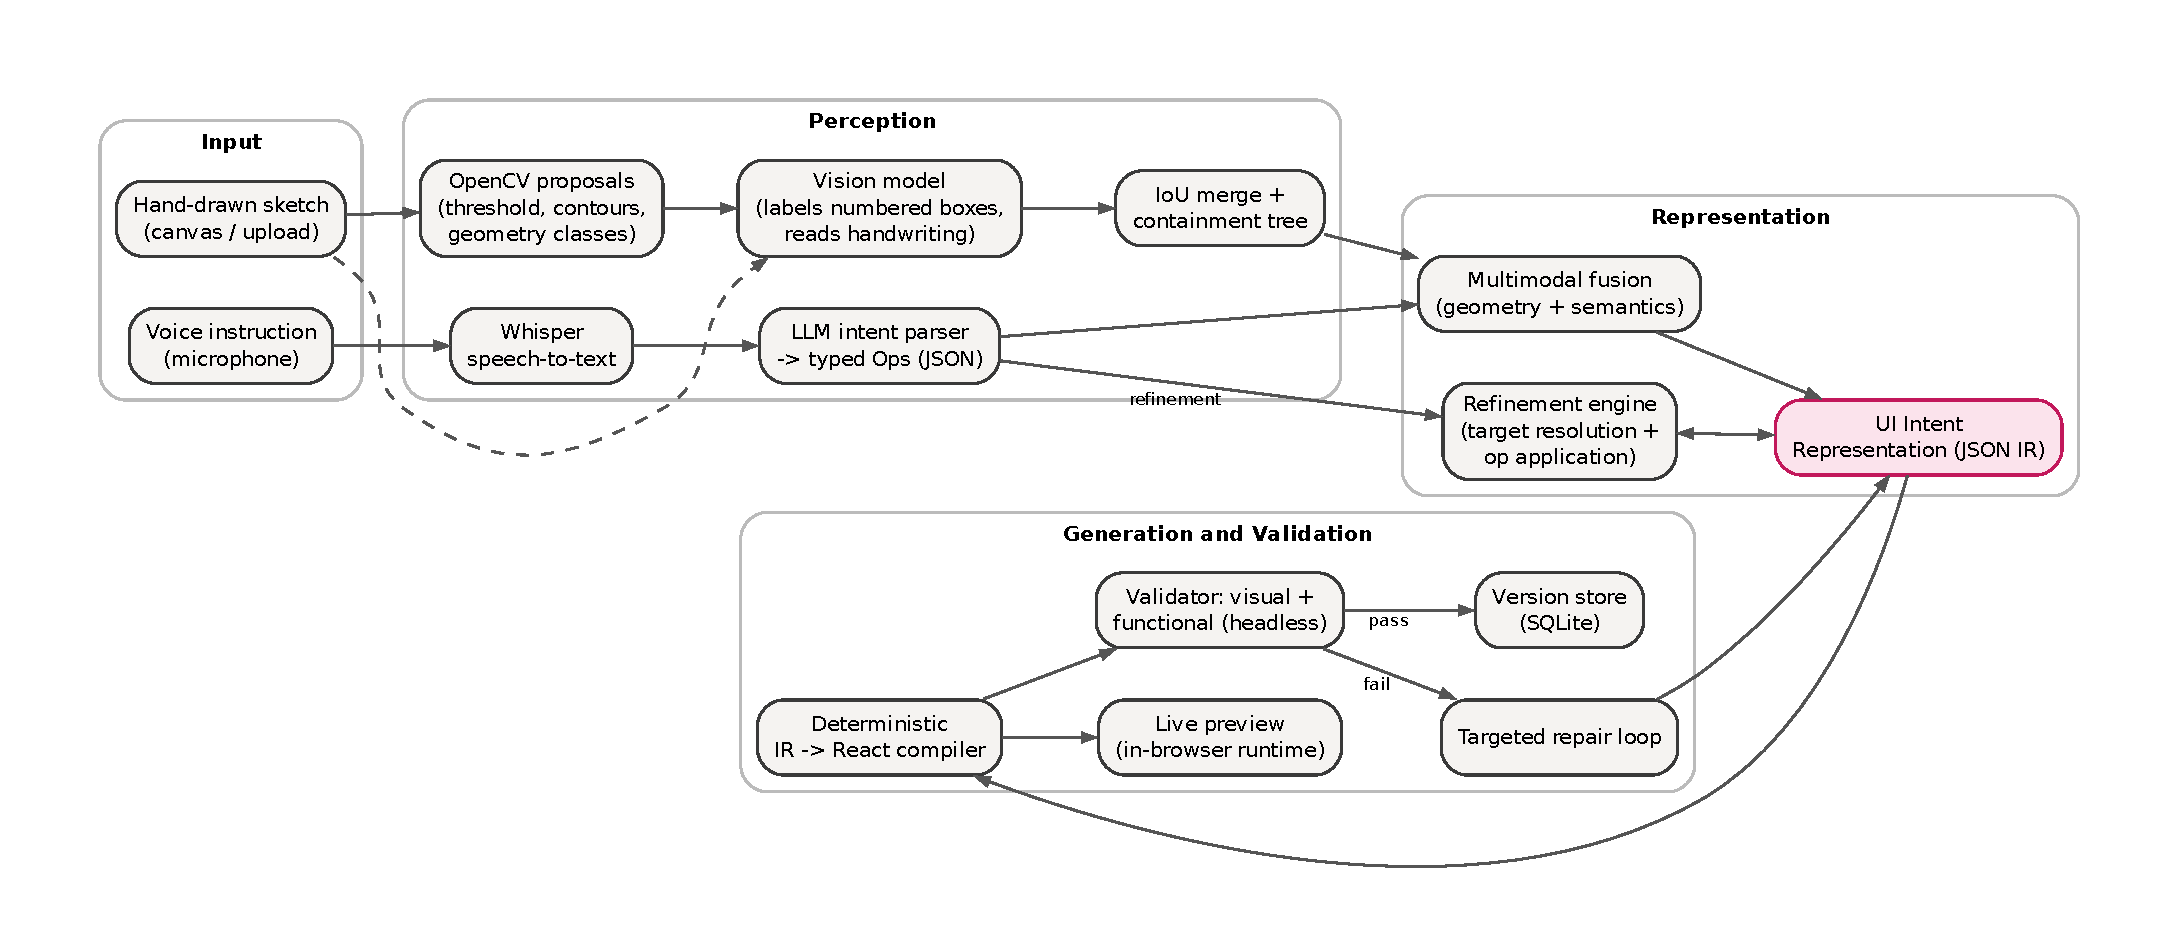
\includegraphics[width=0.92\textwidth]{figures/architecture.pdf}
\caption{NeuroGenUI architecture. Perception (OpenCV proposals, vision labelling, Whisper, LLM intent parsing) feeds a deterministic fusion step that produces the JSON UI Intent Representation (IR). The IR is compiled to React, rendered live, validated in a headless browser and repaired; voice refinements edit the IR rather than regenerating code.}
\label{fig:arch}
\end{figure*}

Fig.~\ref{fig:arch} shows the architecture and Fig.~\ref{fig:flow} the interaction flow. The stages are independent modules with fixed interfaces, each timed separately by the orchestrator (\texttt{upload}, \texttt{analyze\_sketch}, \texttt{transcribe}, \texttt{interpret}, \texttt{fuse}, \texttt{codegen}, \texttt{validate}, \texttt{repair}, \texttt{save}).

\subsection{Sketch Understanding}
\label{sec:sketch}
\textit{OpenCV proposals.} The sketch is converted to grayscale, binarised with adaptive thresholding and closed morphologically so that wobbly, non-closed hand-drawn strokes join into contours. Contours are extracted with their hierarchy~\cite{suzuki1985topological,bradski2000opencv}, approximated by polygons and classified by geometry: small squares become checkbox candidates, small circles radio candidates, wide short rectangles input or button candidates, rectangles crossed by diagonals image placeholders, long thin strokes dividers, and clusters of small strokes handwritten text.

\textit{Vision labelling.} The candidate boxes are drawn with numeric tags onto a copy of the sketch, and a vision model (GPT-4.1-mini) receives this annotated image. Under a JSON schema it assigns each numbered box a component type from the IR vocabulary, transcribes its handwritten text, and adds components the proposals missed. The model therefore classifies and reads but does not localise from scratch.

\textit{Merge.} Vision labels are attached to proposals, added components are merged by IoU, and a containment tree assigns parents. Three modes are available for ablation: \texttt{cv} (geometry only), \texttt{vision} (the model alone, boxes included) and \texttt{hybrid} (the proposed combination).

\subsection{Speech and Intent Understanding}
Speech recorded in the browser is transcribed with Whisper (\texttt{whisper-1}). A language model (GPT-4.1-mini, temperature 0, JSON-schema output) converts the transcript into a list of typed \emph{operations}: \texttt{create}, \texttt{add}, \texttt{remove}, \texttt{modify}, \texttt{move}, \texttt{resize}, \texttt{style}, \texttt{interaction} and \texttt{navigation}. When an IR exists, the model sees a compact outline of it (id, type, label, parent) so it can name targets directly. An operation carries a target reference, an optional new component, a relative position (\emph{below}, \emph{above}, \emph{left\_of}, \emph{right\_of}, \emph{inside}), property and style changes, or an event with actions. The model never writes code.

\subsection{UI Intent Representation}
The IR is a JSON document with pages, each holding a component tree. Every node has a stable id, a type (page, container, card, form, header, navbar, nav item, heading, text, link, button, input, textarea, checkbox, radio, select, image, list, divider, icon), a label, type-specific properties (input type, placeholder, required flag, options), style (variant, colour, size, width, alignment), container layout, a normalised bounding box from the sketch, relations to other nodes, and events. Events bind a trigger (click, submit, change) to an ordered list of actions: \texttt{validate\_required}, \texttt{validate\_format}, \texttt{show\_message}, \texttt{navigate}, \texttt{toggle\_visibility} and \texttt{set\_text}.

\subsection{Multimodal Fusion}
Fusion is deterministic. The sketch decides \emph{where} things are: components are grouped into rows by vertical overlap, containment (by box centre) gives parents, side-by-side columns are detected, and drawn plain containers become cards or forms. The voice description decides \emph{what} they are: input types, required flags, events and the page title. Matching runs in two passes. First, spoken and sketched components with near-identical labels are paired globally, and text-like types count as compatible. Second, each remaining spoken component is matched by type compatibility and reading order between its already-anchored neighbours. A spoken component whose label matches a drawn one is never inserted a second time. When drawn and spoken text disagree, the drawn text is kept and the voice contributes properties and behaviour. Unmatched spoken components are inserted next to their spoken neighbours, and unmatched sketched components are kept. Before fusion, the analysis is cleaned: fragments of one handwritten word are merged, duplicate detections of the same text are removed, and labels that contradict the drawn shape fall back to the geometric class.

\subsection{Code Generation and Live Preview}
A deterministic compiler translates the IR into a React project: one reusable component per IR type (\texttt{Button}, \texttt{Field}, \texttt{Heading}, \texttt{Card}, \dots), one component per page, a state-based router, and event handlers that call a small action runtime. The compiler is \emph{geometry-aware}: the page frame (phone or desktop) follows the sketch's aspect ratio, and each node's normalised sketch box becomes widths and offsets proportional to its parent, vertical spacing proportional to the drawing, and drawn heights for images, buttons and boxes. All of this is expressed with flex rows and columns that wrap on narrow screens rather than absolute positioning, so the code stays responsive and readable. Explicit user styles always override geometry. The output is a runnable Vite project that the user can export and edit, plus a single-script form that the browser runtime transpiles with Babel and renders live in an iframe. Because the compiler is deterministic, the same IR always yields the same code, and a local IR edit yields a local code change.

\subsection{Voice-Guided Refinement}
A spoken refinement is transcribed and interpreted into operations against the current IR. Targets are resolved by the id the model supplied when it is valid, otherwise by a deterministic resolver that scores type keywords, fuzzy label similarity, ordinals (``the second button'') and position words. Application is pure: the IR is deep-copied, only targeted nodes change, untouched nodes stay byte-identical, and every operation reports success or a reason for failure. The changed IR is recompiled and the preview refreshes. Every result is stored as a new version with its transcript, operations, IR, code, validation report and stage timings, so iterative refinement can be inspected and restored.

\subsection{Validation and Targeted Repair}
\begin{figure}[t]
\centering
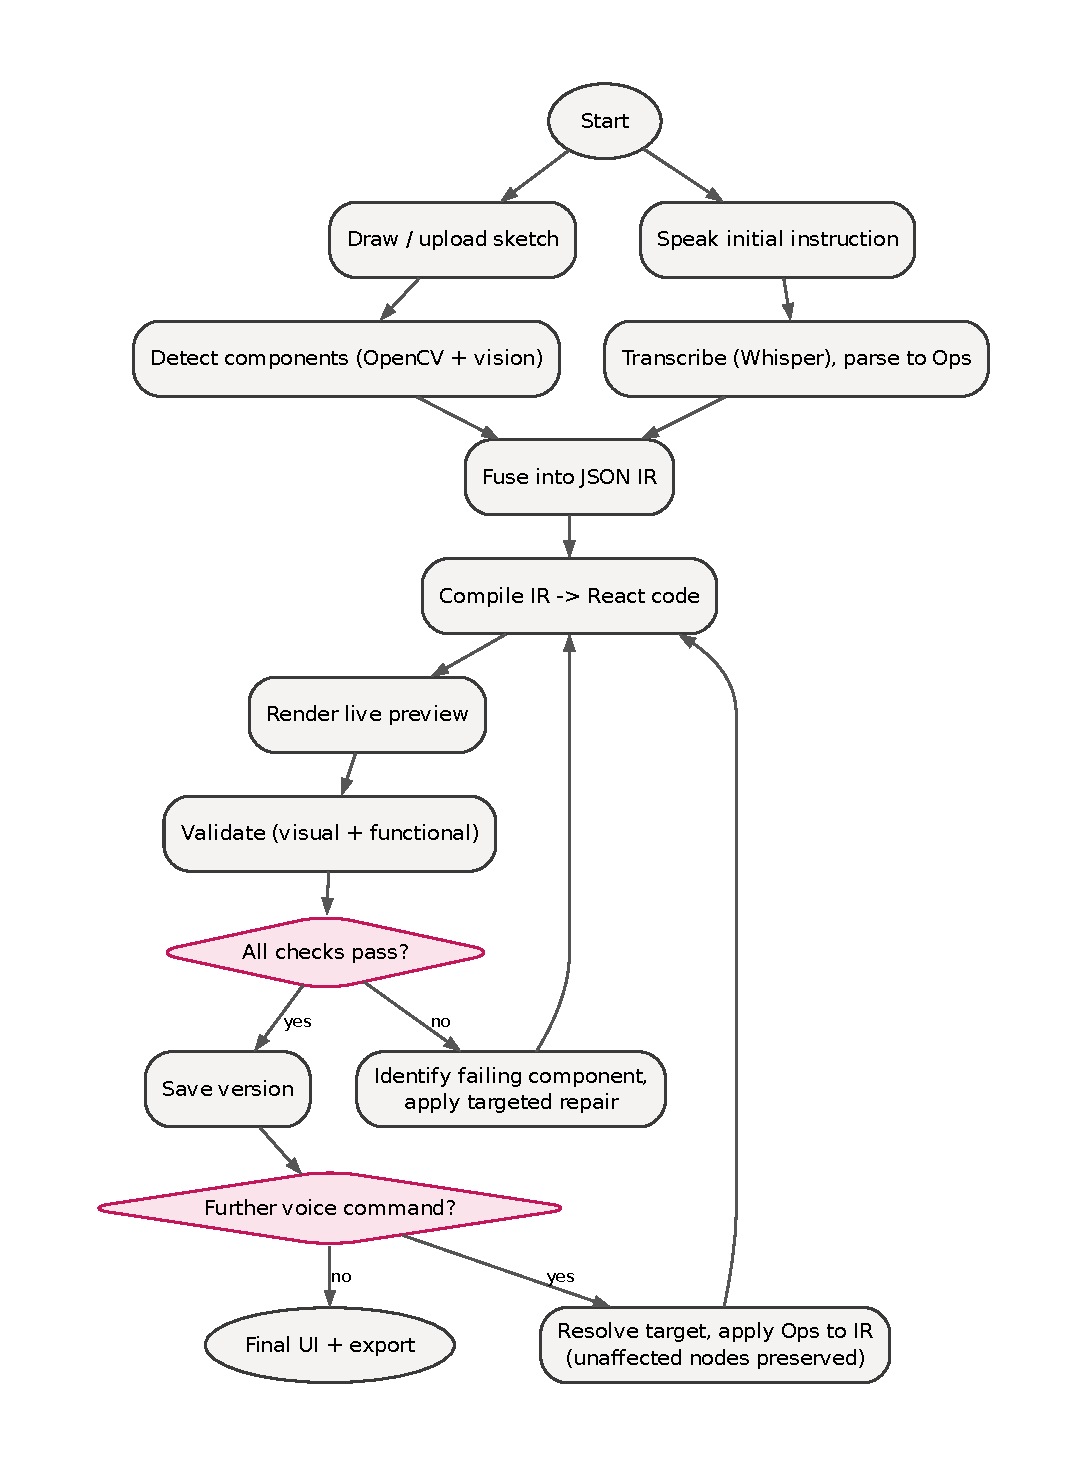
\includegraphics[width=0.78\columnwidth]{figures/flowchart.pdf}
\caption{Interaction flow with validation, targeted repair and iterative voice refinement.}
\label{fig:flow}
\end{figure}
The validator loads the generated code into the same runtime page the user sees, inside a headless browser (Playwright, Chromium or Edge). \textit{Visual checks} verify that every IR node is rendered and visible, that sibling order matches the IR and the sketch, that sketched components are covered, and the overlap between rendered boxes and sketch boxes. \textit{Functional checks} capture runtime and console errors, click every button, type into every input, and simulate every event to assert its effect (an error message for empty required fields, the target page after navigation, a visibility change after a toggle).

The repair loop maps each failing check to the responsible IR node and applies a targeted fix: a missing sketched component is re-inserted from the analysis, out-of-order siblings are reordered, a hidden or zero-size node has its style reset, a node missing from the DOM or a runtime error triggers recompilation in a safe mode, and a failing interaction has its handler rebuilt. The UI is then revalidated, up to three iterations. Repairs never undo an explicit user edit: removed and moved components are recorded in the IR metadata and excluded from coverage and order repairs.
